% \documentclass[aip,jcp,preprint,unsortedaddress,a4paper,onecolum]{revtex4-1}
\documentclass[aip,jcp,a4paper,reprint,onecolumn]{revtex4-1}
% \documentclass[aps,pre,twocolumn]{revtex4-1}
% \documentclass[aps,jcp,groupedaddress,twocolumn,unsortedaddress]{revtex4}

\usepackage[fleqn]{amsmath}
\usepackage{amssymb}
\usepackage[dvips]{graphicx}
\usepackage{color}
\usepackage{tabularx}
\usepackage{algorithm}
\usepackage{algorithmic}

\makeatletter
\makeatother

\newcommand{\recheck}[1]{{\color{red} #1}}
\newcommand{\redc}[1]{{\color{red} #1}}
\newcommand{\bluec}[1]{{\color{blue} #1}}
\newcommand{\greenc}[1]{{\color{green} #1}}
\newcommand{\vect}[1]{\textbf{\textit{#1}}}
\newcommand{\dd}[0]{\textsf{d}}

\newcommand{\AT}{{\textrm{{AT}}}}
\newcommand{\EX}{{\textrm{EX}}}
\newcommand{\CG}{{\textrm{CG}}}
\newcommand{\HY}{{\Delta}}
\newcommand{\rdf}{{\textrm{rdf}}}
\newcommand{\thf}{{\textrm{th}}}
\newcommand{\dof}{{\textrm{dof}}}
\newcommand{\res}{{\textrm{rep}}}
\newcommand{\ext}{{\textrm{extra}}}
\newcommand{\exc}{{\textrm{exc}}}
\newcommand{\thermo}{{\textrm{Q}}}
\newcommand{\hadress}{{\textrm{H}}}
\newcommand{\dadress}{{\textrm{D}}}
\newcommand{\mh}{\mathcal H}
\newcommand{\kin}{\textrm{kin}}
\newcommand{\trans}{\textrm{T}}
\newcommand{\footh}{\textrm{\tiny H}}
\newcommand{\footo}{\textrm{\tiny O}}
\newcommand{\dgenq}{\dot{\underline{\vect q}}}
\newcommand{\dgenp}{\dot{\underline{\vect p}}}
\newcommand{\genq}{{\underline{\vect q}}}
\newcommand{\genp}{{\underline{\vect p}}}


\begin{document}

\title{Calculating the chemical potential by AdResS}
% \author{Han Wang}
% \author{Christof Sch\"utte}
% \author{Luigi Delle Site}
% \affiliation{Institute for Mathematics, Freie Universit\"at Berlin, Germany}

\begin{abstract}
\end{abstract}

\maketitle

\section{The Hamiltonian approach of chemical potential}
We consider the potential interpolation of the
system:
\begin{align}
  U =
  \sum_{i<j} w(\vect R_i) w(\vect R_j)
  U^\AT_{i,j}
  +
  \sum_{i<j}[1- w(\vect R_i) w(\vect R_j)]
  U^\CG_{i,j}
\end{align}
The corresponding intermolecular force is given by
\begin{align}\label{eqn:interpol-f}
  \vect F_{i,j} =
  w(\vect R_i) w(\vect R_j)
  \vect F^\AT_{i,j}
  +
  [1- w(\vect R_i) w(\vect R_j)]
  \vect F_{i,j}^\CG
  -
  \nabla w(\vect R_i) w(\vect R_j)
  (U^\AT_{i,j} - U^\CG_{i,j})
\end{align}
We define the force of changing representation:
\begin{align}
  \vect F_{\res,i} = 
  \sum_j \nabla w(\vect R_i) w(\vect R_j)
  (U^\AT_{i,j} - U^\CG_{i,j})
\end{align}
The difference between the potential interpolation and force
interpolation AdResS is the extra force of
changing representation $\vect F_\res$,
which violates the Newton's
action-reaction law.
The equilibrium of the potential interpolation AdResS
is ensured by the thermodynamic force that is denoted
by $\vect F_\thf^\hadress$.
Throughout this note,
we use the superscript H to indicate this is the thermodynamic force of the
potential interpolation  AdResS, and to distinguish that
of the force interpolation AdResS (standard AdResS)
that is denoted by superscript D.
With the potential interpolation, we can write down
the \emph{global} Hamiltonian for the \emph{whole} system.
By coupling this system
to the Langevin thermostat, we can safely write the Boltzmann
distribution for the system, i.e.  $\frac 1Ze^{\beta\mh}$.  Since the
potential interpolation reduces to the AT and CG potentials in the AT and
CG regions,
% by assuming the filter is infinitely thin,
we approximately
write the fixed-number partition function (like the eq.(16) of the old prove)
\begin{align}
  q(N, V, T)
  \approx
  \frac1{N!}\int\dd\vect x_1\dd\vect x_3\,
  e^{\mh(\vect x_1, N_1, \vect x_3, N_3) +  N_1(\omega^\hadress_\thf + \omega_\dof)}
  =
  \frac1{N!}\int\dd\vect x_1\dd\vect x_3\,
  e^{\mh^\AT_{N_1}(\vect x_1) +\mh^\CG_{N_3}( \vect x_3) +
  N_1(\omega^\hadress_\thf + \omega_\dof)}
\end{align}
$\omega^\hadress_\thf$ is the energy contribution due to the integral
of the thermodynamic force.
$\omega_\dof$ is the energy
given by the thermostat, when turning on extra degrees of freedom in
the AT region. For rigid water system, $\omega_\dof = \frac32
k_BT$. Following the same argument of the old proof, we have
\begin{align}\label{eqn:mueq-h}
  \omega^\hadress_\thf + \omega_\dof = \mu_\CG - \mu_\AT
\end{align}
We will show
later the Hamiltonian approach only provides us with theoretical convenience
for writing down the canonical partition function of the system, in
practice, the traditional force interpolation AdResS is more
applicable. We will also show later the relation between the AdResS of
potential interpolation and force interpolation.
For the force interpolation AdResS, the chemical potential difference 
(provided in the new manuscript) is
\begin{align}\label{eqn:mueq-d}
  \omega^\dadress_\thf + \omega_\dof + \omega_\thermo^\ext = \mu_\CG - \mu_\AT  
\end{align}
The work of the thermostat is composed by two parts: $\omega_\dof +
\omega_\thermo^\ext$. The second term is the extra work of the
thermostat, which comes from the lack of energy conservation due to
the force interpolation, and the different interaction in different
resolution regions. They was not counted by the old manuscript, and shown in
the new manuscript to be crucial for measuring the chemical potential.
% \redc{Here, the new proof is basically the same as the old one, the
%   difference is at the very beginning: the force interpolation
%   AdResS is lack of a global
% Hamiltonian, one cannot safely \emph{assume} the Boltzmann distribution
% of the {whole} system, i.e., the 1st line of Eq~(16) of the old proof is
% problematic.}
\\

\noindent
Now assume an infinitesimal increment of the volume $\Delta V$ of the
AT region, and the same decrement of the volume $-\Delta V$ of the CG
region.  The volume of the hybrid region is kept the same,
so it is a ``piston''
moves toward the CG region by $\Delta L$,
where we assume $\Delta V = \Delta L\cdot A$, where $A$ is the
cutting surface area.
Please also notice by this infinitesimal change of volume, one can
guarantee no molecules changes resolution.
Therefore, the change of the free energy of the system is
\begin{align}
  \Delta A \approx
  A_\AT(N_1, V_1+\Delta V, T) +
  A_\CG(N_3, V_3-\Delta V, T) -
  \int\dd x\, \rho_0 A\cdot \Delta L\cdot
  \Big[
  \vect F^\hadress_\thf(x) -
  \big\langle \vect F_\res(x)\big\rangle
  \Big]
\end{align}
The last term comes from the work done on the piston. It is composed by
two parts, the fist is the work done by the thermodynamic force, and the
second is due to 
the force of changing representation, which does not satisfies the Newton's
action-reaction law. The fist and second part of Eq.~\eqref{eqn:interpol-f}
do not contribute, because they obey the Newton's action-reaction law, so
they are self-canceled.
By some straightforward calculations, we have 
\begin{align}\label{eqn:peq-d}
  \Delta A \approx
  -p_\AT\Delta V + p_\CG\Delta V -
  \rho_0 \Delta V (\omega_\thf^\hadress - \omega_\res)  
\end{align}
Where $ \omega_\res$ is the work of changing representation,
\begin{align}
  \omega_\res
  = \int\dd x\,\langle \vect F_\res (x)\rangle
  = \int\dd x\,\nabla\omega(x)\,
  \big\langle \omega\, (U^\AT - U^\CG)\big\rangle_x
\end{align}
In equilibrium, $\Delta A / \Delta V = 0$ yields
\begin{align}\label{eqn:peq-h}
  \rho_0 (\omega_\thf^\hadress - \omega_\res) = p_\CG - p_\AT
\end{align}
For the force interpolation AdResS, by definition, we have
\begin{align}\label{eqn:peq-d}
  \rho_0\, \omega_\thf^\dadress  = p_\CG - p_\AT  
\end{align}
The superscript D indicate the work is of the force interpolation AdResS.
From Eq.~\eqref{eqn:peq-h} and \eqref{eqn:peq-d}, we have the relation between
the potential interpolation and force interpolation AdResS:
\begin{align}\label{eqn:hd-rel}
  \omega_\thf^\hadress - \omega_\res =  \omega_\thf^\dadress 
\end{align}
From Eq.~\eqref{eqn:mueq-h}, \eqref{eqn:mueq-d} and \eqref{eqn:hd-rel}, we
find the extra work of the thermostat being identical to the work of changing
representation:
\begin{align}
  \omega_\thermo^\ext = \omega_\res
\end{align}
Since the force of changing representation has always the same
direction as $-\nabla w$, and so does the thermodynamic force, the
above equation indicates that the force of changing representation is
actually canceled by the thermodynamic force in the potential
interpolation AdResS, and ends up the same simulation as the force
interpolation AdResS. This indicates a much stronger statement than Eq.~\eqref{eqn:hd-rel}:
\begin{align}
  \vect F_\thf^\hadress - \langle\vect F_\res\rangle = \vect F_\thf^\dadress
\end{align}
This relation is numerically checked by the AdResS water simulation, please see Fig.~\ref{fig:tmp1}.
\begin{figure}
  \centering
  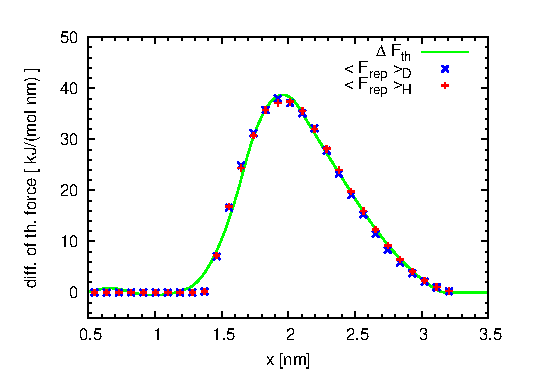
\includegraphics[]{fig/diff.thf/diff-thf.eps}
  \caption{The difference between the thermodynamic force of the
    potential interpolation-based scheme and force interpolation of the standard AdResS.
    The green solid line shows the difference of the thermodynamic
    forces, i.e. $\Delta{\vect F}_\thf={\vect F}_\thf^\hadress-{\vect F}_\thf^\dadress$.
    The blue and red symbols indicate the quantity $\langle \vect F_\res\rangle = \langle w\nabla w(U^{\AT}-U^{\CG})\rangle$ calculated in the two different approaches (blue corresponds to the standard AdResS while red to the Hamiltonian-based approach). The equivalence between the two approaches is suggested by the fact that $\Delta{\vect F}_\thf$ corresponds to $\langle \vect F_\res\rangle$, and that this latter is actually the same independently from the approach used to calculate it.}
  \label{fig:tmp1}
\end{figure}
In practice, the force interpolation AdResS has
the convenience of systematically improve the accuracy,
so it is much more favorable than the potential interpolation
AdResS. In comparison, the potential interpolation AdResS
shown here only has the first order of accuracy (only the density is
fixed by the $\vect F_\thf^\hadress$), and the systematical accuracy
improvement looks complicated.


\section{Numerical tests}

\subsection {Spherical model system}
We test the model system: in AT region are spherical molecules
interacting with the $r^{-12}$ potential, while in the CG region are
spherical molecules interacting with the WCA potential. Clearly,
the energy from the thermostat is $\omega_\dof = 0$.
\begin{itemize}
\item check Eq.~\eqref{eqn:mueq-h}
  \begin{align}
  &\mu_\CG - \mu_\AT = 23.0 - 55.4 = -32.4 \,\textsf{kJ/mol}\\
  &\omega^\hadress_\thf + \omega_\dof = \omega^\hadress_\thf= -33.0  \,\textsf{kJ/mol}
  \end{align}
\item check Eq.~\eqref{eqn:peq-d}
  \begin{align}
    &p_\CG - p_\AT = (9627.52 - 22251.6) \,\textsf{Bar} / \rho_0 = - 22.8  \,\textsf{kJ/mol} \\
    &\omega^\dadress_\thf = - 23.3  \,\textsf{kJ/mol}
  \end{align}
\item check Eq.~\eqref{eqn:hd-rel}
  \begin{align}
    &\omega^\hadress_\thf - \omega^\dadress_\thf = -9.7 \,\textsf{kJ/mol}\\
    &\omega_\res = -9.8 \,\textsf{kJ/mol} \quad \textrm{measured by potential interpol. AdResS}\\
    &\omega_\res = -9.8 \,\textsf{kJ/mol} \quad \textrm{measured by force interpol. AdResS}
  \end{align}
\end{itemize}

\subsection{Water system}
The result of the water system is:
\begin{itemize}
\item check Eq.~\eqref{eqn:mueq-h}
  \begin{align}
    &\mu_\CG - \mu_\AT = (-19.3 + 23.0) - (-19.3-9.7-23.5) = 56.2 \,\textsf{kJ/mol}\\
    &\omega^\hadress_\thf + \omega_\dof = 51.6 + 3.8 = 55.4  \,\textsf{kJ/mol}
  \end{align}
\item check Eq.~\eqref{eqn:peq-d}
  \begin{align}
    &p_\CG - p_\AT = (9627.52 - 350.1) \,\textsf{Bar} / \rho_0 = 16.8  \,\textsf{kJ/mol} \\
    &\omega^\dadress_\thf = 16.6  \,\textsf{kJ/mol}
  \end{align}
\item check Eq.~\eqref{eqn:hd-rel}
  \begin{align}
    &\omega^\hadress_\thf - \omega^\dadress_\thf = 34.9 \,\textsf{kJ/mol}\\
    &\omega_\res = 35.0 \,\textsf{kJ/mol} \quad \textrm{measured by potential interpol. AdResS}\\
    &\omega_\res = 34.6 \,\textsf{kJ/mol} \quad \textrm{measured by force interpol. AdResS}
  \end{align}
\end{itemize}


% \begin{align}
%   &\mu_\CG - \mu_\AT = (-19.3 + 23.0) - (-19.3-9.7-23.5) = 56.2 \,\textsf{kJ/mol}\\
%   &\omega^\hadress_\thf + \omega_\dof = 52.4 + 3.8 = 56.2  \,\textsf{kJ/mol}\\
%   &p_\CG - p_\AT = (9627.52 - 350.1) \,\textsf{Bar} / \rho_0 = 16.8  \,\textsf{kJ/mol} \\
%   &\omega^\dadress_\thf = 16.6  \,\textsf{kJ/mol}\\
%   &\omega^\hadress_\thf - \omega^\dadress_\thf = 35.8 \,\textsf{kJ/mol}\\
%   &\omega_\res = 34.4 \,\textsf{kJ/mol} \quad \textrm{measured in potential interpol. AdResS}
% \end{align}





\end{document}





